\section{Множественные и пространственные отношения на графах}

\mysubsection{Операции над графами}

	Если вы решаете сложную задачу, то эффективно сначала разбить ее на подзадачи, потом решить их, а в заключение объединить результаты в общий ответ. Похожая ситуация появляется в тот момент, как вы решаете анализировать граф: вы сначала разбиваете его на подграфы, анализируете их, а потом уже получаете искомый результат. 
	
	Чтобы упростить этот подход, были введены обозначения и операции над графами, которые в некотором виде повторяют операции над множествами и отображениями.
	
	Представим, что у вас есть два графа $G_1(V_1, E_1)$ и $G_2(V_2, E_2)$, притом в этом случае мы уже рассматривает их не с точностью до изоморфизма, а так, будто их вершины и ребра пронумерованы. Тогда можно задать тривиальную операцию \emph{объединения графов $G_1$ и $G_2$}:
	$$G_1 \cup G_2 = G(V_1 \cup V_2, E_1 \cup E_2).$$
	
	При объединении графов никаких дополнительных ребер не появляется и все те ребра, которые были хотя бы в одном из графов, остаются в них. В противоположность такой операции можно представить, что графы $G_1$ и $G_2$ расположены на двух параллельных плоскостях и, говоря о \emph{соединении графов} (обозначается $G_1 + G_2$), мы будем подразумевать, что каждую вершину графа $G_1$ мы совединяет ребром с каждой вершиной графа $G_2$.
	
	Чтобы еще сильнее сокращать записи, будем писать вместо $\bigcup\limits_{i=1}^{k} G$ просто $kG$.
	
	Продолжая аналогию с операциями над множествами, можно ввести \emph{декартово произведение графов $G_1$ и $G_2$}, взяв при этом в качестве множества вершин $V = V_1 \times V_2$, а ребрами соединив вершины $a = (a_1, a_2)$ и $b = (b_1, b_2)$ в том и только том случае, если $a_1$ смежна $b_1$ или $a_2$ смежна $b_2$.
	
	Также можно ввести еще одну бинарную операцию, которая уже не поддается простой аналогии с предыдущими операциями, "--- \emph{композицию графов $G = G_1[G_2]$}. Под ней мы будем подразумевать граф, в котором так же $V = V_1 \times V_2$, но ребром соединены вершины $a = (a_1, a_2)$ и $b = (b_1, b_2)$ тогда и только тогда, когда $a_1$ смежна $b_1$ или $a_1 \equiv b_1$ и $a_2$ и $b_2$ смежны.  
	
	В этих обозначениях легко, например, определить \emph{полный $n$-дольный граф $K(\alpha_1, \dots, \alpha_n)$} как следующее соединение
	$$K(\alpha_1, \dots, \alpha_n) = \overline{K_{\alpha_1}} + \overline{K_{\alpha_2}} + \dots + \overline{K_{\alpha_n}}.$$
	
	Также $Q_k$, то есть $k$-кубы, можно определить рекрсивно $Q_k = Q_{k-1} \times K_2$. 
	
\mysubsection{Метрика на графах}

	Как мы увидим в самых поздних частях этой книги, граф обладает многими интересными свойствами, связанными с его изображениями в пространствах. Но даже на том уровне, который мы сейчас имеем, можно уже определить некоторые метрические понятия на графах.

\begin{definition}
	\emph{Расстоянием $d(a, b)$ между вершинами $a$ и $b$} называется длина наименьшего пути, соединяющего их.
\end{definition}
	
	Заметим, что такой путь всегда простой. Кроме того, чтобы это понятие распространялось на несвязные графы, принято считать, что для несвязанных вершин $c$ и $e$ расстояние $d(c, e) = \infty$.

	По сути такое определение расстояния на графе задает метрику на нем. Давайте точнее определим это понятие.
	
\begin{definition}
	Множество $M$ вместе с введенным на нем бинарным отображением $\rho \colon M \times M \to \BR_{\geqslant 0}$ называется \emph{метрическим пространством}, если \emph{метрика} (то есть то самое отображение $\rho$) удовлетворяет трем свойствам:
	\begin{itemize}
		\item $\forall \!\ a, b \in M \mapsto \rho (a, b) \geqslant 0, \rho (a, b) = 0 \Leftrightarrow a \equiv b$ (неотрицательность),
		\item $\forall \!\ a, b \in M \mapsto \rho (a, b) = \rho (b, a)$ (коммутативность),
		\item $\forall \!\ a, b, c \in M \mapsto \rho (a, b) + \rho (b, c) \geqslant \rho (a, c)$ (неравенство треугольника).
	\end{itemize}
\end{definition}

	В случае с нашими графами расстояние принимает только дискретные значения $(0, 1, 2, 3, \dots)$, но это не мешает ему удовлетворять всем трем свойствам. И поэтому такое определение расстояния задает метрику на нашем графе.
	
	Для новичков: не стоит бояться этих мудренных слов, суть метрического пространства только в том, что для заданного отображения выполнены три свойства, которые интуитивно понятны для традиционного пространства $\BR^2$ "--- евклидова плоскость. Действительно, если мы зададим в качестве метрики кратчайшее расстояние между двумя точками плоскости, то первое свойтсво эквивалентно неотрицательности длины отрезка, второе "--- независимости выбора концов отрезка в качестве первой и второй точки, третье "--- даже по названию одноименному неравенству, доказываему в курсе школьной геометрии.
	
	Как и в любом пространстве задаются окрестности, так и здесь можно задать \emph{$\epsilon$-окрестность вершины $a$} (обозначается $U_{\epsilon}(a)$) как максимальный подграф $G(V')$, порожденный множеством вершин $V' \subset V$ такое, что $\forall \!\ b \in V' \mapsto d(a, b) \leqslant \epsilon$. Обратите внимание, что мы работаем с замкнутыми окрестностями, что вообще не свойственно для них.
	
\begin{center}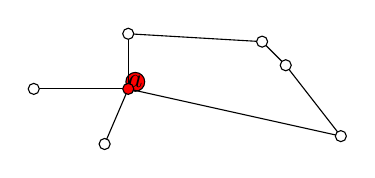
\begin{tikzpicture}
	\draw (0, 0) node [above right] {$a$};	

	\tikzstyle{every node}=[circle, draw, fill=white, inner sep=0pt, minimum width=4pt]	
	
	\draw (0, 0) -- (0, 0.7);
	\draw (0, 0) -- (-1.2, 0);
	\draw (0, 0) -- (-0.3, -0.7);
	
	\draw (0, 0.7) -- (1.7, 0.6) -- (2, 0.3) -- (2.7, -0.6) -- (0, 0);
	
    \draw (-1.2, 0) node {}
    	  (0, 0.7) node {}
    	  (2.7, -0.6) node {}
    	  (-0.3, -0.7) node {}
    	  (1.7, 0.6) node {}
    	  (2, 0.3) node {};	
    	  
	\tikzstyle{every node}=[circle, draw, fill=red, inner sep=0pt, minimum width=4pt]

	\draw (0, 0) node {};	
\end{tikzpicture} \;\ \;\ \;\ 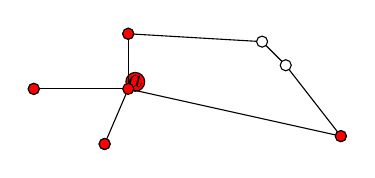
\begin{tikzpicture}
	\draw (0, 0) node [above right] {$a$};	

	\tikzstyle{every node}=[circle, draw, fill=white, inner sep=0pt, minimum width=4pt]	
	
	\draw (0, 0) -- (0, 0.7);
	\draw (0, 0) -- (-1.2, 0);
	\draw (0, 0) -- (-0.3, -0.7);
	
	\draw (0, 0.7) -- (1.7, 0.6) -- (2, 0.3) -- (2.7, -0.6) -- (0, 0);
	
    \draw (-1.2, 0) node {}
    	  (0, 0.7) node {}
    	  (2.7, -0.6) node {}
    	  (-0.3, -0.7) node {}
    	  (1.7, 0.6) node {}
    	  (2, 0.3) node {};	
    	  
	\tikzstyle{every node}=[circle, draw, fill=red, inner sep=0pt, minimum width=4pt]

	\draw (0, 0) node {};	
	
	\draw (-1.2, 0) node {}
    	  (0, 0.7) node {}
    	  (2.7, -0.6) node {}
    	  (-0.3, -0.7) node {};	
\end{tikzpicture} \;\ \;\ \;\ 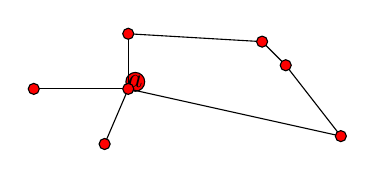
\begin{tikzpicture}
	\draw (0, 0) node [above right] {$a$};	

	\tikzstyle{every node}=[circle, draw, fill=white, inner sep=0pt, minimum width=4pt]	
	
	\draw (0, 0) -- (0, 0.7);
	\draw (0, 0) -- (-1.2, 0);
	\draw (0, 0) -- (-0.3, -0.7);
	
	\draw (0, 0.7) -- (1.7, 0.6) -- (2, 0.3) -- (2.7, -0.6) -- (0, 0);	
    	  
	\tikzstyle{every node}=[circle, draw, fill=red, inner sep=0pt, minimum width=4pt]

	\draw (0, 0) node {};	
	
	\draw (-1.2, 0) node {}
    	  (0, 0.7) node {}
    	  (2.7, -0.6) node {}
    	  (-0.3, -0.7) node {}
    	  (1.7, 0.6) node {}
    	  (2, 0.3) node {};	
\end{tikzpicture}\end{center}
\begin{center}
	\small Рис. \images. Слева-направо нарисован граф с отмеченными соответственно $U_0 (a)$, $U_1 (a)$, $U_2 (a)$
\end{center}

	Ясно, что это не единственная метрика, которую можно задать на графах. Также можно задать тривиальную метрику, которую называют \emph{дискретной метрикой}, которая задается следующим образом
	$$\rho (a, b) = 0 \Leftrightarrow a \equiv b, \rho (a, b) = 1 \Leftrightarrow a \not\equiv b \;\ \forall \!\ a, b \in V.$$

	Кроме того, мы в разделе про орграфы говорили об эквивалентности, которую можно ввести на графах, "--- о сильной связности. И фактически мы получим схожую с дискретной метрикой \emph{метрику достижимости}, которая ставит ноль тем парам вершин, которые связаны, и единицу в противном случае

\mysubsection{Эксцентриситет, радиус, диаметр}

	Сейчас мы повторим мучительный путь, совершенный в начале второй главы, где пришлось на нескольких страницах познакомиться с большим числом определений. Здесь это также необходимо, чтобы все утверждения и задачи, которые мы решим, имели не слишком длинные формулировки. Начнем же!

\begin{definition}
	\emph{Эксцентриситетом вершины $a$} называется максимальное расстояние от этой вершины до вершин графа, то есть
	$$\epsilon(a) = \max\limits_{b \in V} d(a, b).$$
\end{definition}

\begin{definition}
	Максимальный и минимальный элемент множества эксцентриситетов графа называется соответственно \emph{радиусом графа} и \emph{диаметром графа}
	$$r(G) = \min\limits_{a \in V} \epsilon(a), \;\ d(G) = \max\limits_{a \in V} \epsilon(a).$$
\end{definition}

	Так как везде мы рассматриваем конечные графы, то вполне тривиально доказывается, что радиус и диаметр достигаются на вершинах графа, то есть существуют хотя бы по одной из следующих вершин.
	
\begin{definition}
	\emph{Центральная вершина} "--- вершина, у которой эксцентриситет равен радиусу. \emph{Периферийная вершина} "--- вершина, у которой эксцентриситет равен диаметру графа.
\end{definition}
	
	И в этот момент интуиция читателя может сломаться, потому что в общем случае нет единственности центральной и периферийной вершины.
	
\begin{statement}
	В любом связном графе есть хотя бы две периферийные вершины.
	
\begin{proof}
	Как мы заметили выше, в графе есть периферийная вершина $a$, тогда по определению есть минимальный простой путь, соединяющий $a$ и какую-то другую вершину $b$, длины $d(G)$. Тогда $\epsilon(b) \geqslant d(G)$, следовательно, так как $d(G)$ "--- максимальный эксцентриситет, то имеет место точное равенство $\epsilon(b) = d(G)$. Это и означает, что вершина $b$ "--- тоже периферийная вершина. Все, мы нашли две периферийные вершины.
\end{proof}
\end{statement}	

	С центральной вершиной все сложнее: например, в графах $P_n$ число центральных вершин быдет чередоваться между $1$ и $2$. А у графов $C_n$ все вершины будут одновременно и периферийными и центральными.

\begin{statement}
	Удаленностью вершины дерева назовём сумму расстояний от неё до всех остальных вершин. Докажите, что в дереве, у которого есть две вершины с удаленностями, отличающимися на 1,~---~нечётное число вершин.
	
\begin{proof}
	Допустим противное и прийдем к противоречию.
		
	Рассмотрим две смежные вершины $a, b$. Тогда кроме них есть еще четное число вершин. Если мы посмотрим на разность удаленностей этих двух вершин, то заметим, что это будет сумма четного числа $1$ и $-1$. Достаточно просто можно проверить, что такая сумма всегда четная. Следовательно, удаленности смежных вершин имеют одинаковую четность. 
	
	Как инвариант относительно смежности вершин четность удаленности вершин можно распространить на все вершины и получить, что любые две вершины дерева должны иметь удаленности не отличающиеся по четности, что неверно по условию. Противоречие.
\end{proof}
\end{statement}

	Заметим, что обратное утверждение неверно. Для этого достаточно рассмотреть граф-звезду с $n \geqslant 4$ вершинами.	
	
\mysubsection{Задачи}

\begin{exersize}
	Пусть в графе $G$ $45$ вершин и степень каждой из них не меньше $22$. Докажите, что любые две вершины $a$ и $b$ графа $G$ либо смежны, либо $d (a, b) = 2$. 
\end{exersize}	

\begin{exersize}[Омельченко А. В. <<Теория графов>>]
	Докажите, что радиус и диаметр графа связаны следующим образом:
	$$r(G) \leqslant diam (G) \leqslant 2r(G).$$
	Приведите примеры графов, на которых оба неравенства достигаются.
\end{exersize}

\begin{exersize}[Омельченко А. В. <<Теория графов>>]
	Докажите, что в простом графе с $\Delta = n-2$ и диаметром $2$
	количество ребер $m \geqslant 2n - 4$.
\end{exersize}

\begin{exersize}[Агаханов Н.Х., Богданов И.И., Кожевников П.А., Подлипский О.К., Терешин Д.А. <<Всероссийские олимпиады школьников по математике 1993~---~2009: Заключительные этапы>>]
	В стране $1993$ города, и из каждого выходит не менее $93$ дорог. Известно, что из любого города можно проехать по дорогам в любой другой. Докажите, что это можно сделать не более, чем с $62$ пересадкамию (Дорога соединяет между собой два города.)
\end{exersize}	 

\begin{exersize}[Агаханов Н.Х., Богданов И.И., Кожевников П.А., Подлипский О.К., Терешин Д.А. <<Всероссийские олимпиады школьников по математике 1993~---~2009: Заключительные этапы>>]
	В стране некоторые пары городов соединены дорогами, которые не пересекаются вне городов. В каждом городе установлена табличка, на которой указана минимальная длина маршрута, выходящего из этого города и проходящего по всем остальным городам страны (маршрут может проходить по некоторым городам больше одного раза и не обязан возвращаться в исходный город). Докажите, что любые два числа на табличках отличаются не более, чем в полтора раза.
\end{exersize}	  

